\documentclass[12pt]{report}
\usepackage[a4paper,bindingoffset=0.2in,%
left=1in,right=1in,top=1in,bottom=1in,%
footskip=.25in]{geometry}
\usepackage[affil-it]{authblk}
\usepackage[utf8]{inputenc}
\usepackage{listings}
\usepackage{color}
\usepackage{xcolor}
\usepackage{pdfpages}
\usepackage{graphicx}
\usepackage{textcomp}
\usepackage{hyperref}
\usepackage{dirtree}

\definecolor{codegreen}{rgb}{0,0.6,0}
\definecolor{codegray}{rgb}{0.5,0.5,0.5}
\definecolor{codepurple}{rgb}{0.58,0,0.82}
\definecolor{backcolour}{rgb}{1.0,1.0,1.0}

\newcommand{\folder}[2]{}


\lstdefinestyle{mystyle}{
	backgroundcolor=\color{backcolour},   
	commentstyle=\color{codegreen},
	keywordstyle=\color{magenta},
	numberstyle=\tiny\color{codegray},
	stringstyle=\color{codepurple},
	basicstyle=\scriptsize,
	breakatwhitespace=false,         
	breaklines=true,                 
	captionpos=b,                    
	keepspaces=true
}
\lstset{style=mystyle}

\begin{document}
	\title{%
		0SumBot\\[1ex]
		
\includegraphics[width=64pt,height=12pt]{badge.png}
	}
	\author{Aly Shmahell\\%
		\href{aly.shmahell@gmail.com}{aly.shmahell@gmail.com}
	}
	\affil{%
		3rd Year Student\\
		Department of Computer Science, University of L'Aquila\\
		Computational Intelligence in Videogames and Virtual Reality
		}
	\date{December 18, 2017}
	
	\maketitle
	\begin{abstract}
		0SumBot can be described as a sum of two varied approaches to create a bot capable of playing, and sometimes, preferably most times, winning the PlanetWars contest.\\
		In this effort The need to optimize parameters lead to the creation of 0SumBot, 1SumBot, G0Bot and G0GA.
			\end{abstract}

	\section{\textbf{General Description}}
		0SumBot depends on the following in-game variables: Planet.NumShips(), Planet.GrowthRate(), PlanetWars.Distance(Planet,otherPlanet).\\
		In order to achieve victory first we set a series of optimized versions of these parameters and compare them to the in-game parameters and then we set (Base, Target, FleetSize) based on the results.\\
		One way of comparison is by calculating the localMinima of distance between base and enemy planets, and basing our choice of target on the result.\\
		Another method that is followed is comparing each planet directly to optimized parameters to formulate a plan of attack.\\
		Methods of comparison are not totally exclusive, and we usually use them entwined.\\
		1SumBot is an alteration of 0SumBot that includes a localMinima for (Base, Enemy), (Base, Neutral) and (Base, Ally), then changes the strategy to include these additional parameters.\\
		G0Bot is a copy of 0SumBot used for the G0GA genetic algorithm.\\
		G0GA is a genetic algorithm designed for the purpose of fine-tuning the parameters of G0Bot for a more efficient battle strategy.
\section{Notes on the bots}
In order to avoid player timeout, make sure to check if planet is null before you make any operation involving that selected planet.\\
For example, when calculating local minima in 0SumBot it is essential to perform the following check beforehand:
\begin{lstlisting}[language=Java]
if(closestEnemy==null)
	return;
localMinima =  pw.Distance(base,closestEnemy);
\end{lstlisting}
		\newpage
		\section{\textbf{file description}}
		\setlength{\DTbaselineskip}{20pt}
		\DTsetlength{1em}{3em}{0.1em}{1pt}{4pt}
		\renewcommand*\DTstylecomment{\ttfamily\color{blue}}
		\newcommand*\DTstyleunimportant{\ttfamily\color{gray}}
		\renewcommand*\DTstyle{\ttfamily\color{red}}
		\dirtree{%
			.1 PlanetWars-0SumBot.
			.2 G0GA.py: \DTstylecomment{the genetic algorithm code (written in pure python 2.7)}.
			.2 fitOnot: \DTstylecomment{shellscript used for commencing fitness testing on G0Bot}.
			.2 winner.txt \DTstylecomment{used to store battle result to be read by G0GA}.
			.2 grun: \DTstylecomment{shellscript for compiling and running G0Bot}.
			.2 G0Bot.
			.3 G0Bot.java.
			.3 \DTstyleunimportant{....}.
			.2 run: \DTstylecomment{shellscript for compiling and running 0SumBot}.
			.2 crun: \DTstylecomment{shellscript for compiling PlanetWars, example-bots and 0SumBot, then running 0SumBot}.
			.2 0SumBot.
			.3 zeroSumBot.java.
			.3 oneSumBot.java.
			.3 \DTstyleunimportant{....}.
			.2 documentation: \DTstylecomment{folder housing documentation material}.
			.2 AlyShmahell-0SumBot.pdf: \DTstylecomment{final documentation file}.
			.2 \DTstyleunimportant{PlanetWars-viz: the PlanetWars source-code}.
			.2 \DTstyleunimportant{3rdPartBots}.
			.2 \DTstyleunimportant{exampleBots}.
			.2 \DTstyleunimportant{maps}.
			.2 \DTstyleunimportant{rmv-dbg.py}.
			}
\newpage
	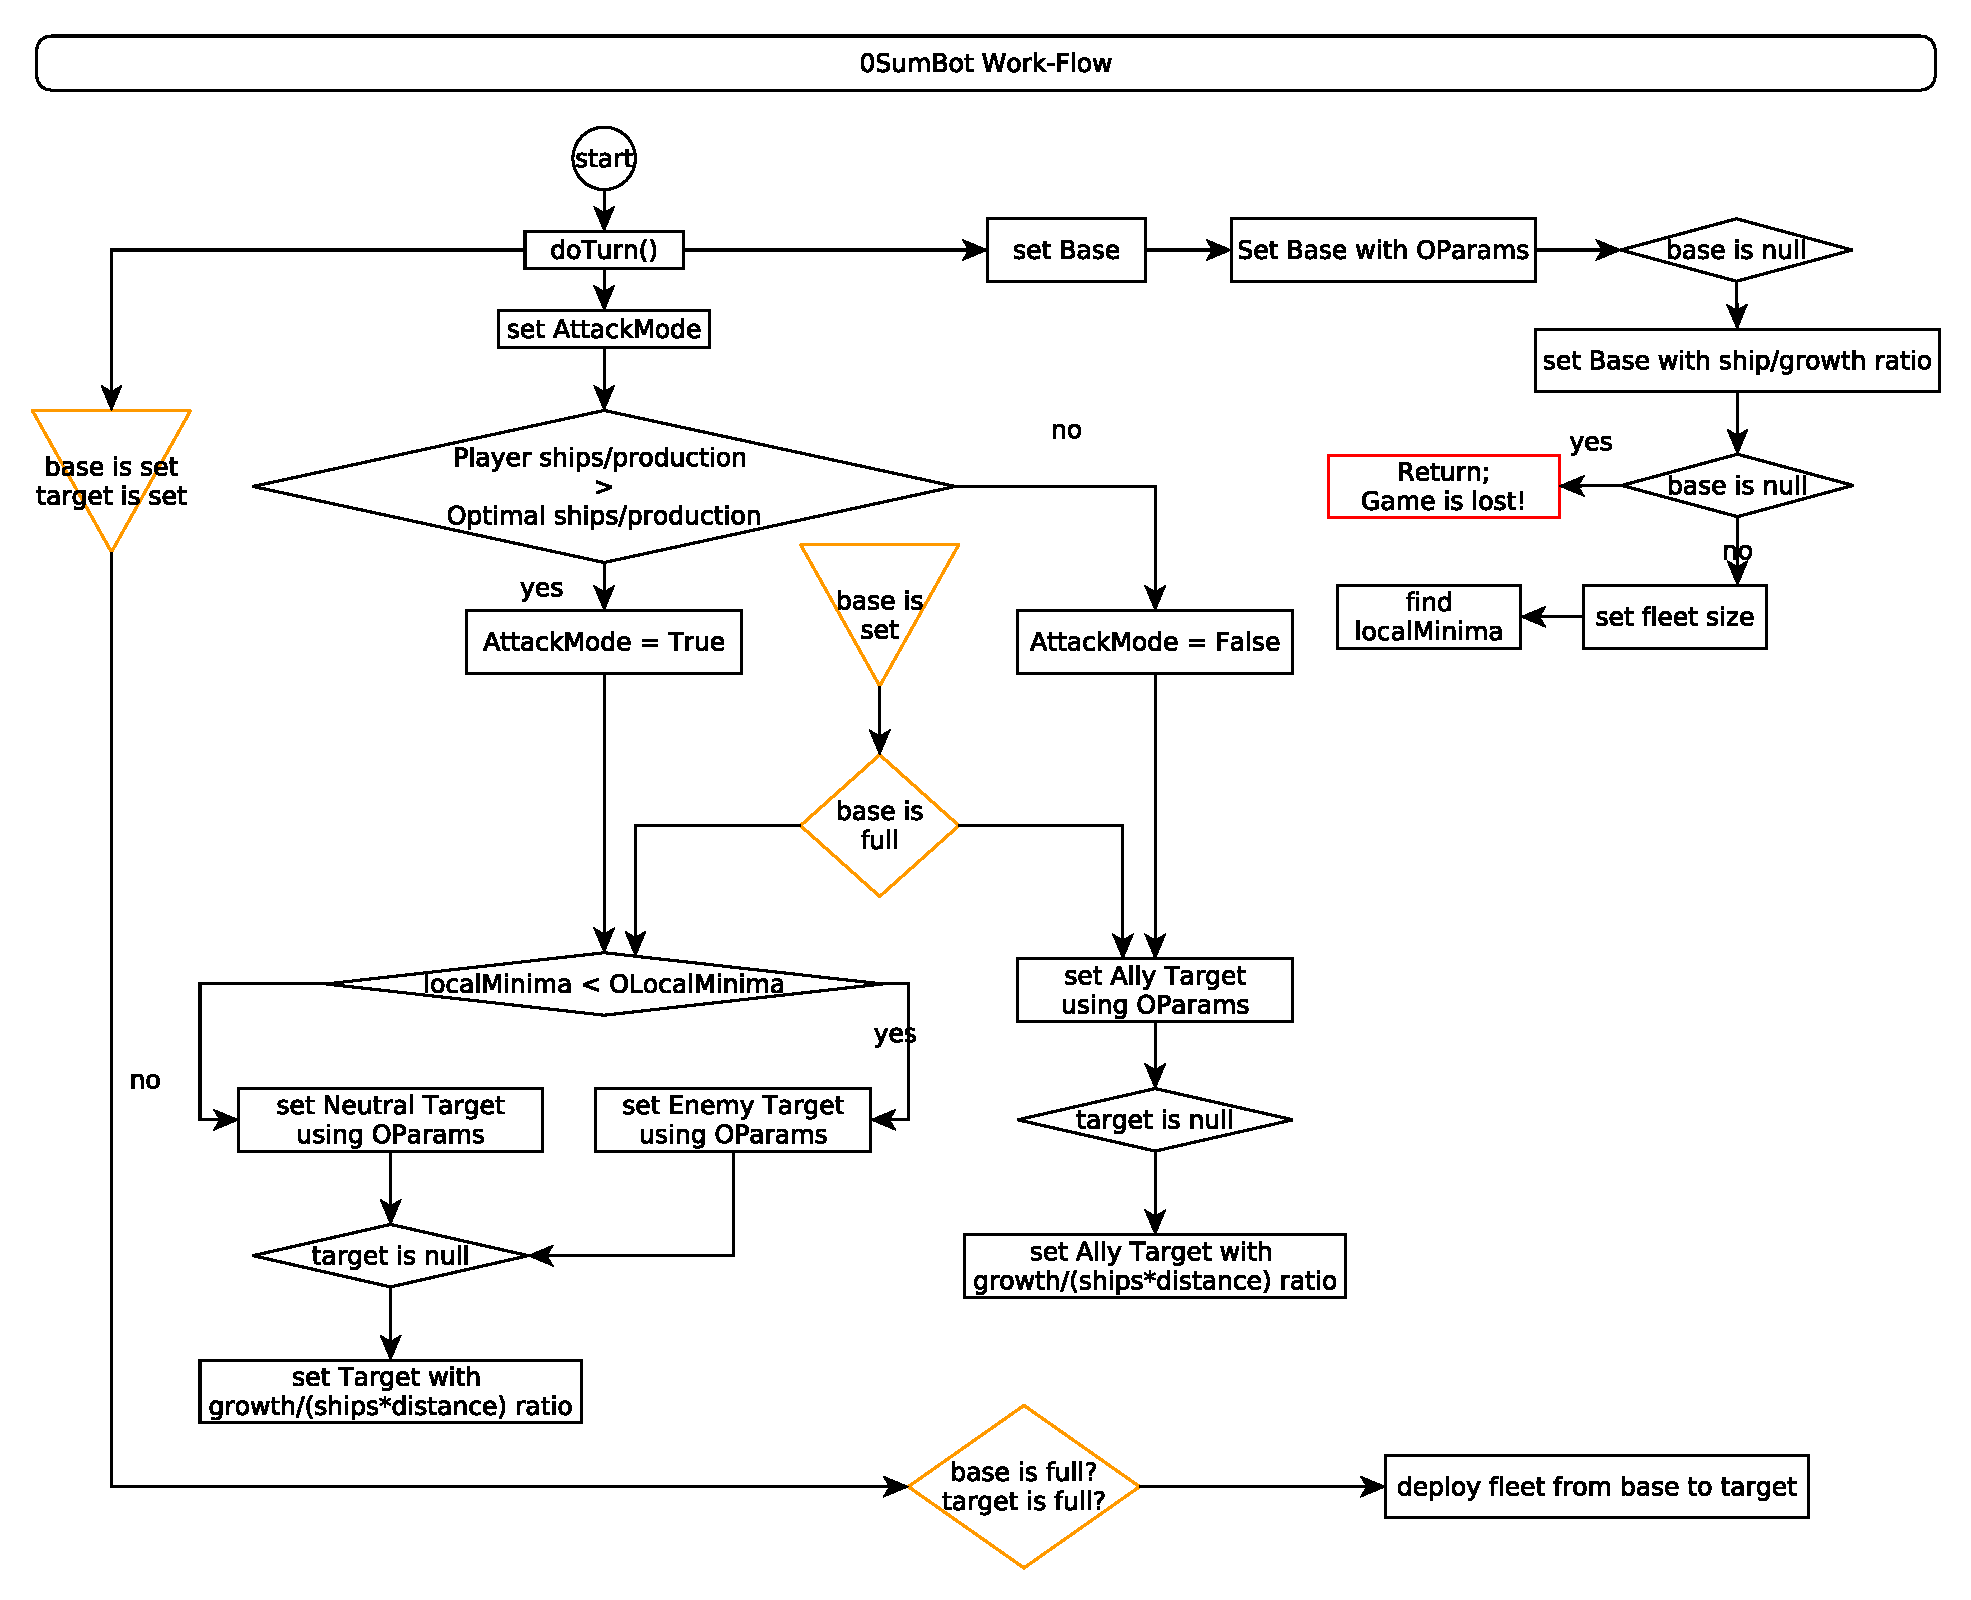
\includepdf[pagecommand={\section{0SumBot} \thispagestyle{empty}}]{0SumBot.pdf}
\newpage
	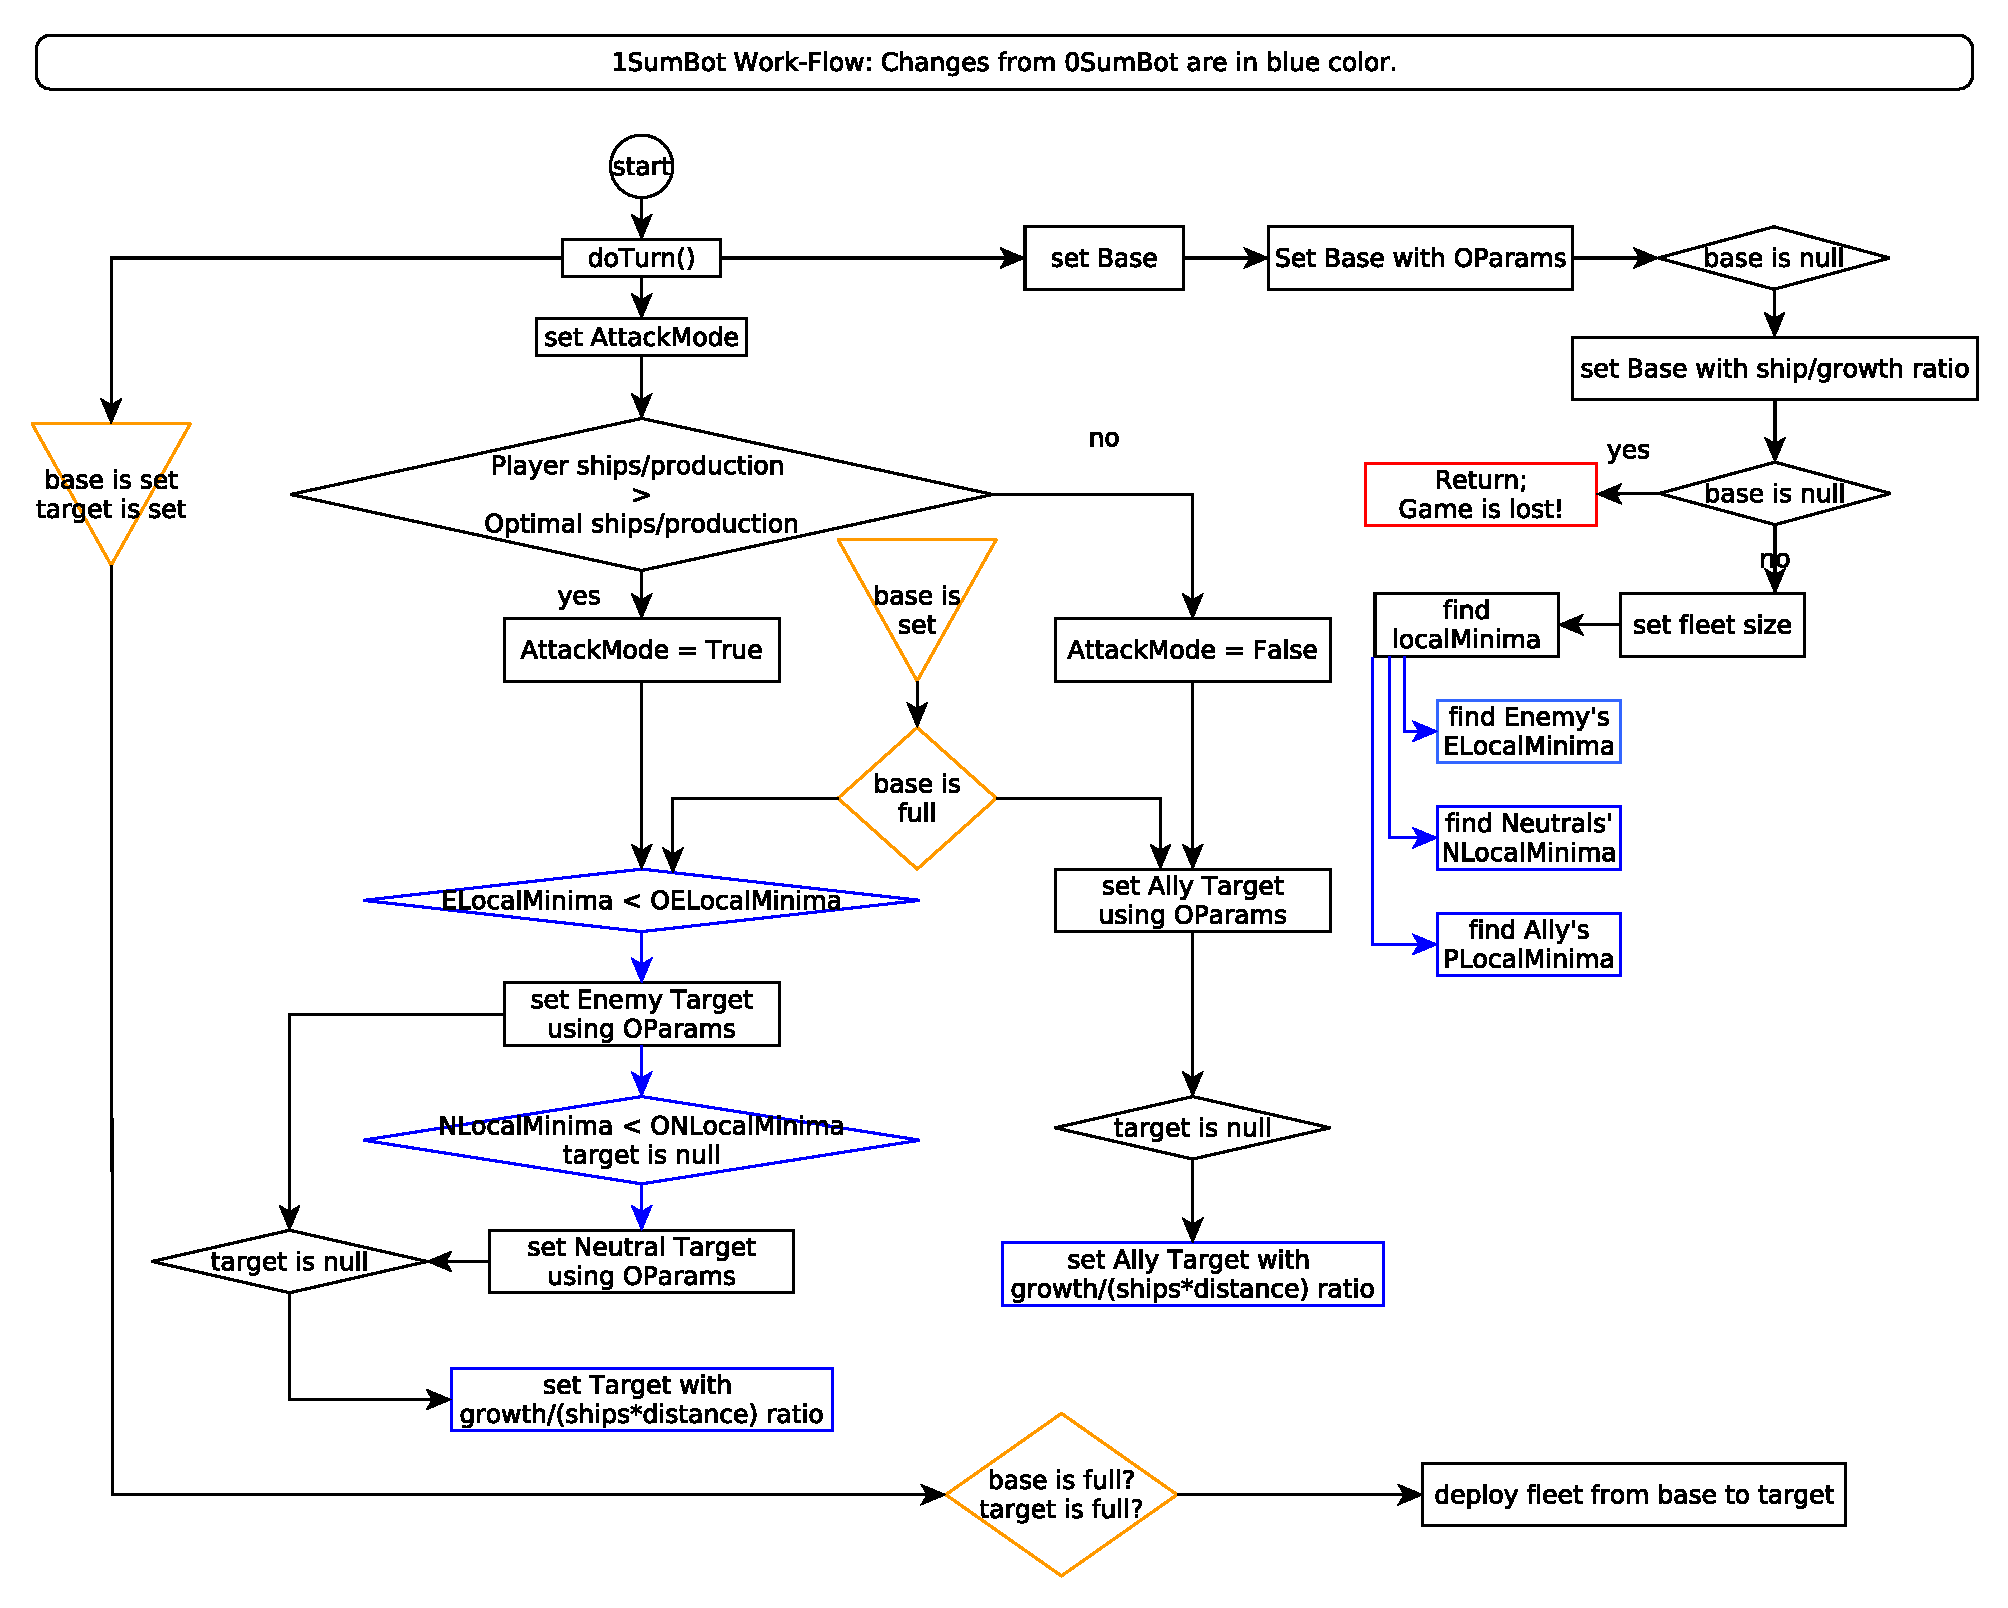
\includepdf[pagecommand={\section{1SumBot} \thispagestyle{empty}}]{1SumBot.pdf}
\newpage
	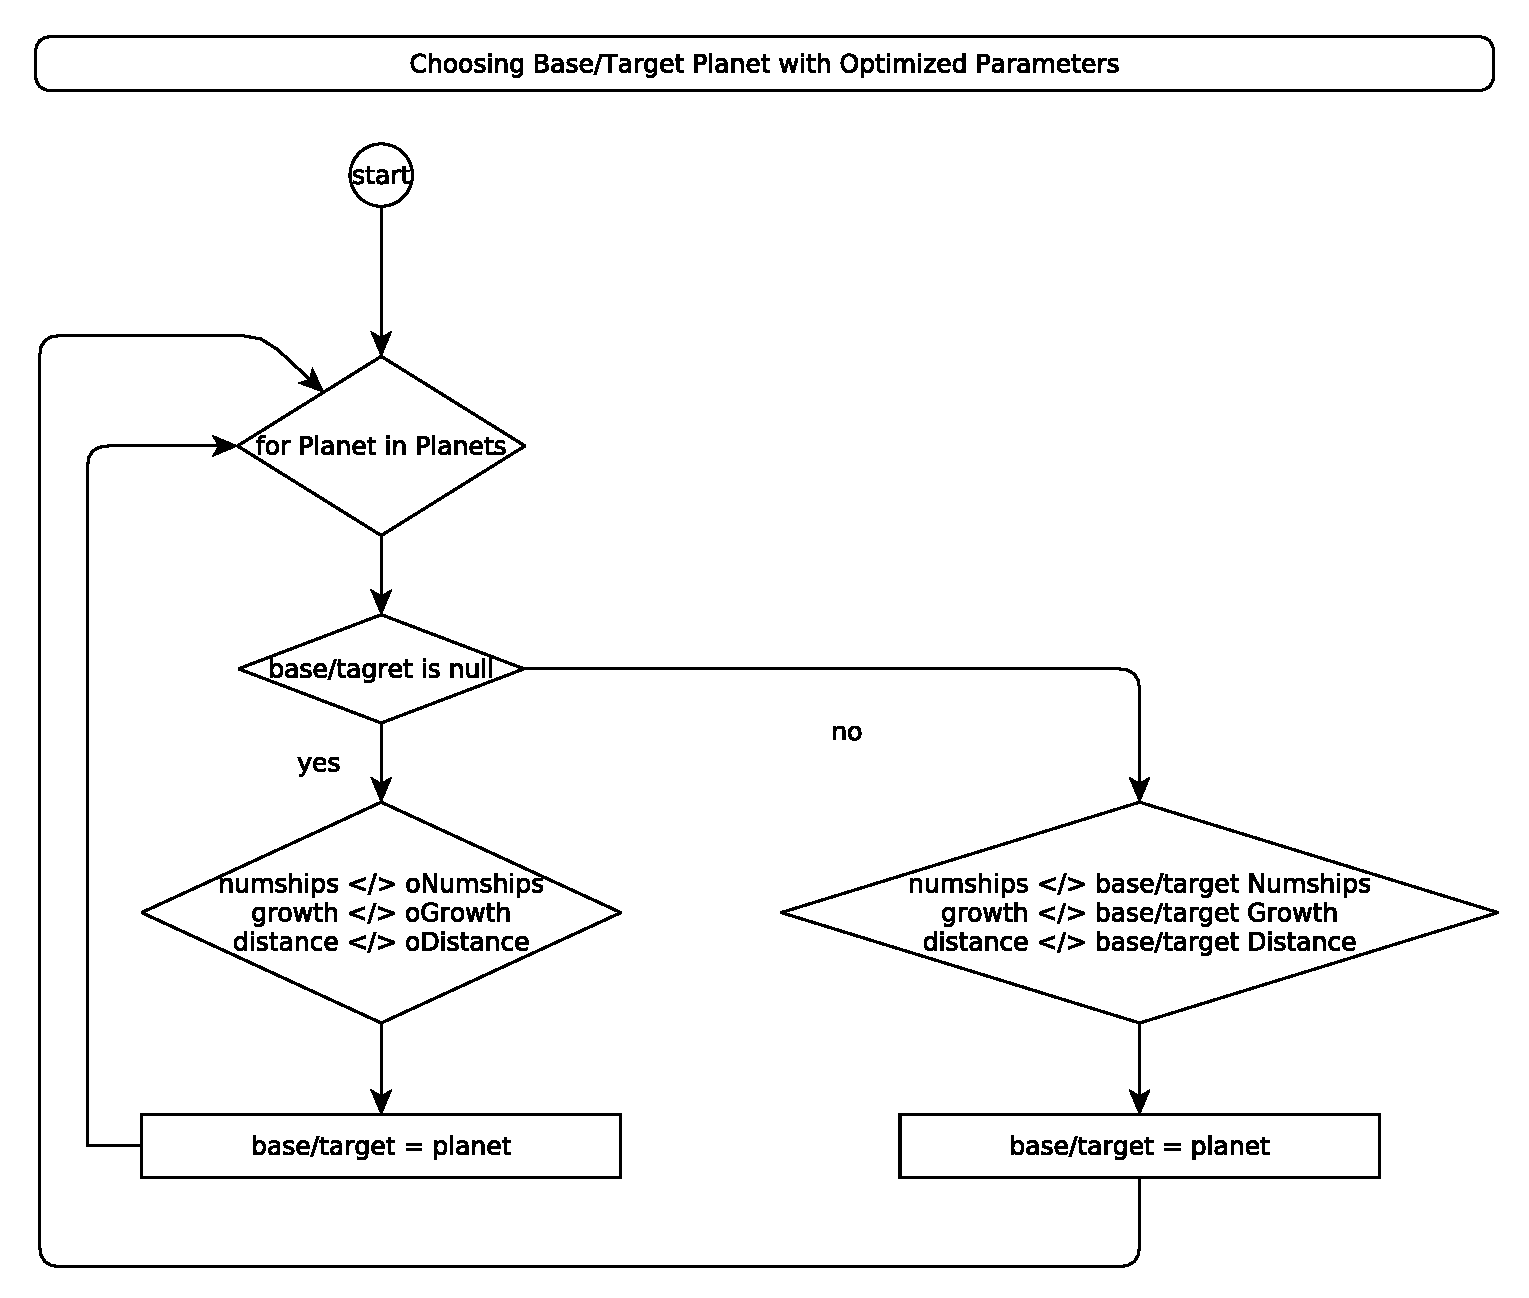
\includepdf[pagecommand={\section{\normalsize{Choosing planet according to optimized parameters}} \thispagestyle{empty}}]{setPlanetOParams.pdf}
	\newpage
		\newpage
		\section{G0GA}
		G0GA is a steady-state 4-k tournament genetic algorithm improvised to evolve G0Bot.\\
		Written in python 2.7, it performs fitness calculation by means of multiple bot simulations aided by helper bash scripts.\\
		The GA performs parameter passing to the bot and to the helper scripts by means of line replacement directly on the target files (parameter injection).\\
		\subsection{Notes on the GA}
		Always make sure to run as few calls to fitness as possible, in order to reduce simulation time and therefor decrease computation time.\\
		This can be achieved by:\\
			\begin{itemize}
				\item Inside the generation generator	: 
				\begin{itemize}
					\item Assigning fitness values to fitness variables and reusing them.
					\item Assigning fitness values only when needed.
					\item Only assigning fitness values when no change on the genotype is due later.
				\end{itemize}
				\item Inside the individual: 
				\begin{itemize}
					\item Assigning fitness value to internal default\_fitness variable.
				\end{itemize}
			\end{itemize}
	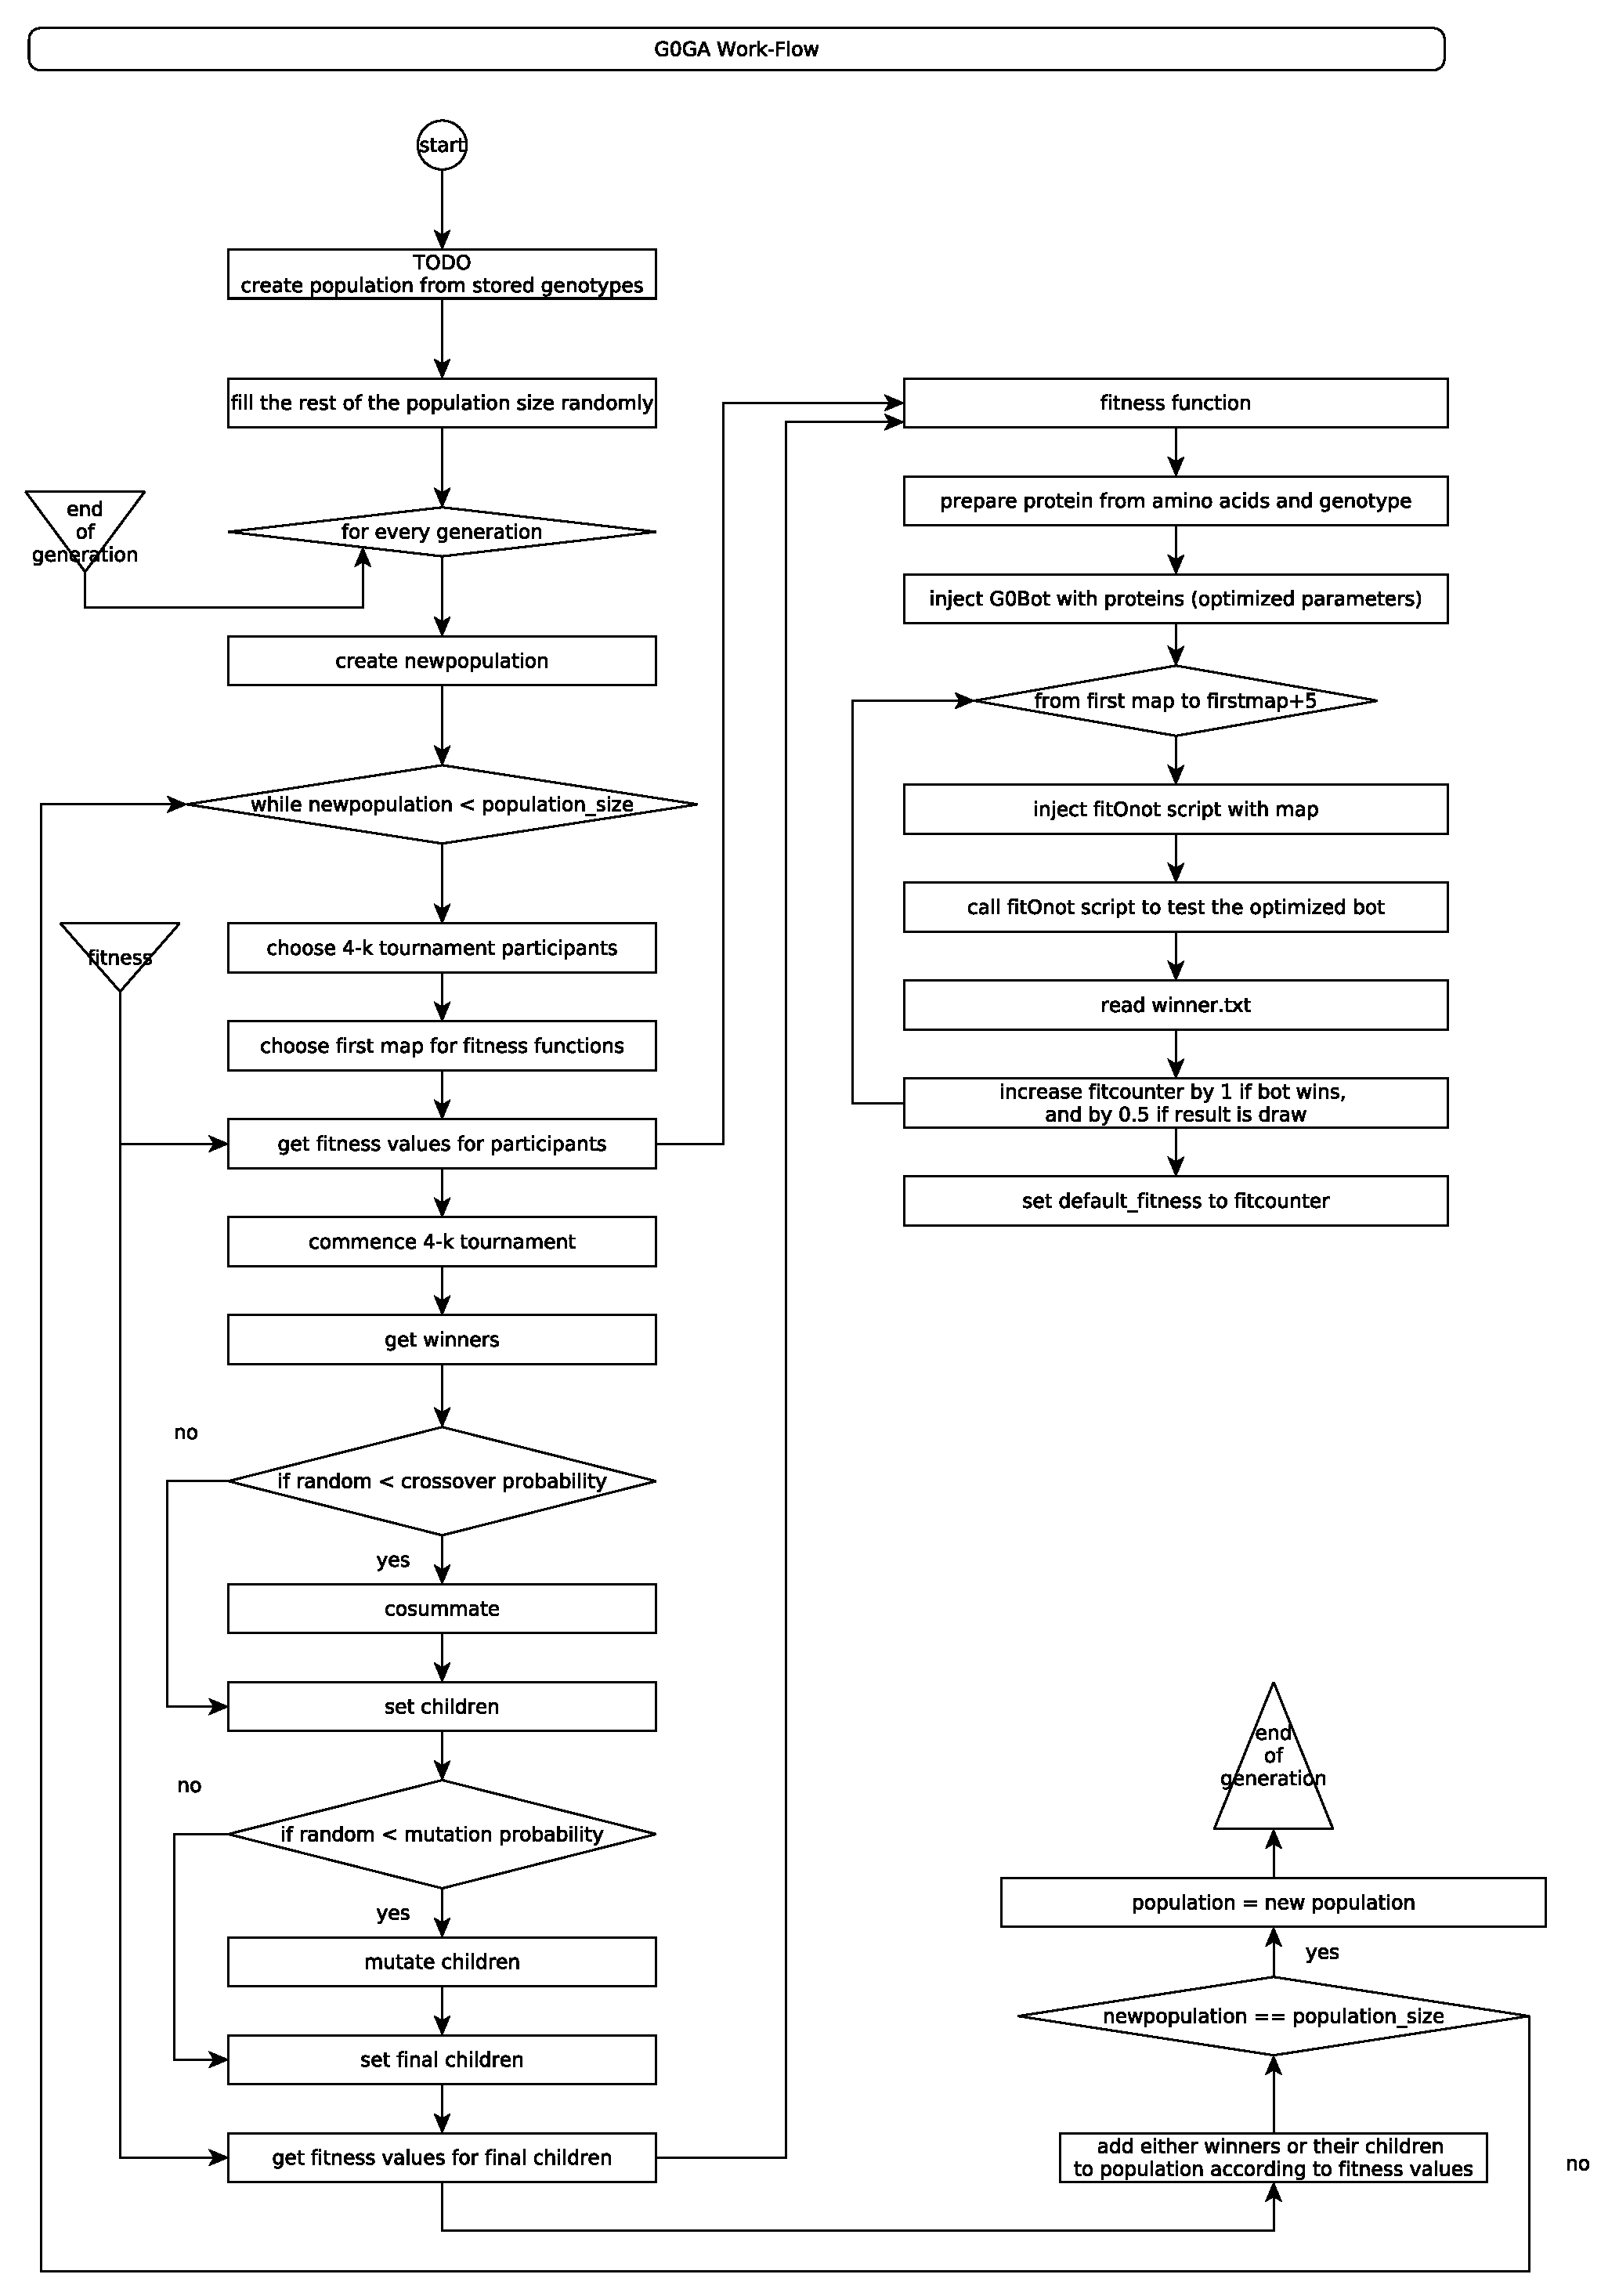
\includepdf{G0GA.pdf}
	\newpage
	\section{What's next?}
	\begin{itemize}
		\item Adding memory capability to G0GA, so that it records the best genotypes from the current run session in order for it to use them in creating individuals for future run sessions.
		\item Using Linear Regression in G0Bot and in G0GA to increase performance.
		\item Redefining battle strategy in G0Bot based on fuzzy functions.
		\item Improving the map shuffling process in G0GA.
		\item Accessing and use more in-game variables in G0Bot, like Fleet variables for example.
	\end{itemize}
\begin{flushleft}
	\section{\textbf{Code Repository}}
\end{flushleft}
\begin{flushleft}
	A Github repository exists for this project under:\\
\end{flushleft}
	\begin{center}
		\url{https://github.com/AlyShmahell/PlanetWars-0Sum}
	\end{center}
\end{document}
